\section{mo\-TSMove\-Loop\-Expl$<$ M $>$ Class Template Reference}
\label{classmo_t_s_move_loop_expl}\index{moTSMoveLoopExpl@{moTSMoveLoopExpl}}
Explorer for a Tabu Search algorithm.  


{\tt \#include $<$mo\-TSMove\-Loop\-Expl.h$>$}

Inheritance diagram for mo\-TSMove\-Loop\-Expl$<$ M $>$::\begin{figure}[H]
\begin{center}
\leavevmode
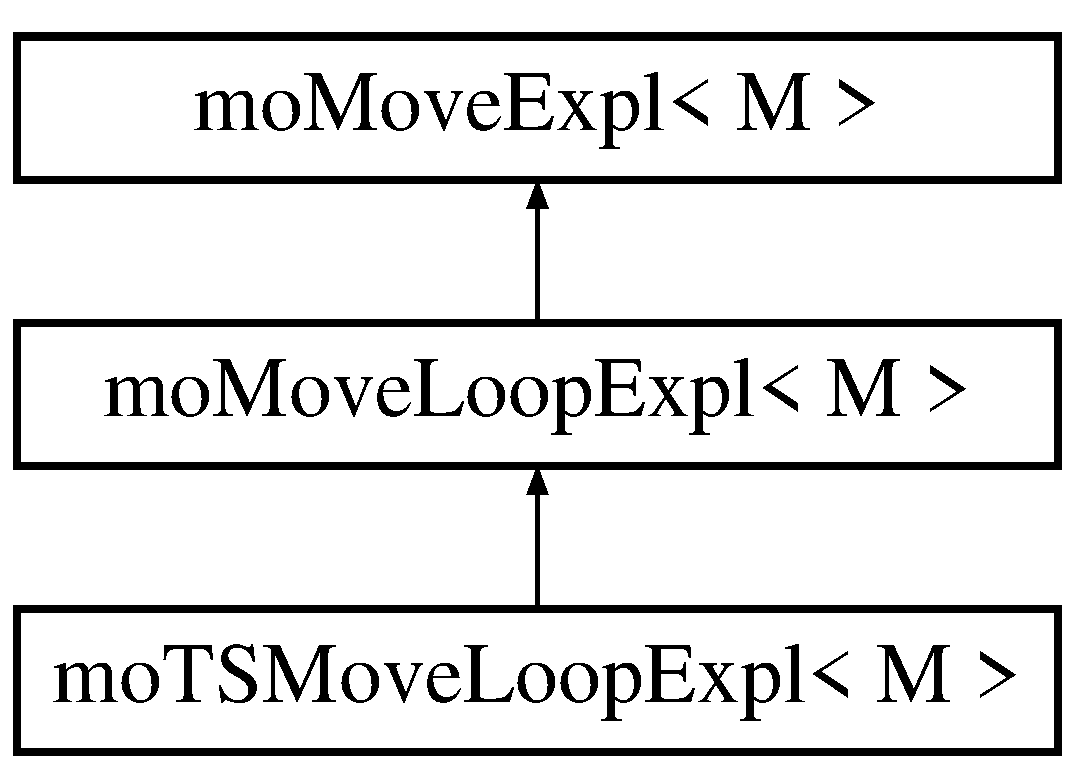
\includegraphics[height=3cm]{classmo_t_s_move_loop_expl}
\end{center}
\end{figure}
\subsection*{Public Member Functions}
\begin{CompactItemize}
\item 
{\bf mo\-TSMove\-Loop\-Expl} ({\bf mo\-Move\-Init}$<$ M $>$ \&\_\-\_\-move\_\-init, {\bf mo\-Next\-Move}$<$ M $>$ \&\_\-\_\-next\_\-move, {\bf mo\-Move\-Incr\-Eval}$<$ M $>$ \&\_\-\_\-incr\_\-eval, {\bf mo\-Tabu\-List}$<$ M $>$ \&\_\-\_\-tabu\_\-list, {\bf mo\-Aspir\-Crit}$<$ M $>$ \&\_\-\_\-aspir\_\-crit)
\begin{CompactList}\small\item\em Constructor. \item\end{CompactList}\item 
void {\bf operator()} (const {\bf EOT} \&\_\-\_\-old\_\-sol, {\bf EOT} \&\_\-\_\-new\_\-sol)
\begin{CompactList}\small\item\em Procedure which lauches the exploration. \item\end{CompactList}\end{CompactItemize}
\subsection*{Private Types}
\begin{CompactItemize}
\item 
typedef M::EOType {\bf EOT}\label{classmo_t_s_move_loop_expl_47f42225e2ed096374b818bdb848a527}

\begin{CompactList}\small\item\em Alias for the type. \item\end{CompactList}\item 
typedef M::EOType::Fitness {\bf Fitness}\label{classmo_t_s_move_loop_expl_a1ba36c937b195ca2f7d1a24adaa7018}

\begin{CompactList}\small\item\em Alias for the fitness. \item\end{CompactList}\end{CompactItemize}
\subsection*{Private Attributes}
\begin{CompactItemize}
\item 
{\bf mo\-Move\-Init}$<$ M $>$ \& {\bf move\_\-init}\label{classmo_t_s_move_loop_expl_6b23f99648902fb72ed17a4a6fa4e400}

\begin{CompactList}\small\item\em Move initialisation. \item\end{CompactList}\item 
{\bf mo\-Next\-Move}$<$ M $>$ \& {\bf next\_\-move}\label{classmo_t_s_move_loop_expl_aeeff6666d26ff5c67acd9c153a5ae49}

\begin{CompactList}\small\item\em Neighborhood explorer. \item\end{CompactList}\item 
{\bf mo\-Move\-Incr\-Eval}$<$ M $>$ \& {\bf incr\_\-eval}\label{classmo_t_s_move_loop_expl_ee4443fc8e45d840697619678628c26c}

\begin{CompactList}\small\item\em Efficient evaluation. \item\end{CompactList}\item 
{\bf mo\-Best\-Impr\-Select}$<$ M $>$ {\bf move\_\-select}\label{classmo_t_s_move_loop_expl_35a3f3035fb8df875c281d9838904bf1}

\begin{CompactList}\small\item\em Move selector. \item\end{CompactList}\item 
{\bf mo\-Tabu\-List}$<$ M $>$ \& {\bf tabu\_\-list}\label{classmo_t_s_move_loop_expl_0e5988a940ba218e87c53b7e56d79790}

\begin{CompactList}\small\item\em Tabu list. \item\end{CompactList}\item 
{\bf mo\-Aspir\-Crit}$<$ M $>$ \& {\bf aspir\_\-crit}\label{classmo_t_s_move_loop_expl_6786cf5422d17cbf872b07ae74ca6b0f}

\begin{CompactList}\small\item\em Aspiration criterion. \item\end{CompactList}\end{CompactItemize}


\subsection{Detailed Description}
\subsubsection*{template$<$class M$>$ class mo\-TSMove\-Loop\-Expl$<$ M $>$}

Explorer for a Tabu Search algorithm. 

It is used by a {\bf mo\-TS}{\rm (p.\,\pageref{classmo_t_s})}. 



Definition at line 30 of file mo\-TSMove\-Loop\-Expl.h.

\subsection{Constructor \& Destructor Documentation}
\index{moTSMoveLoopExpl@{mo\-TSMove\-Loop\-Expl}!moTSMoveLoopExpl@{moTSMoveLoopExpl}}
\index{moTSMoveLoopExpl@{moTSMoveLoopExpl}!moTSMoveLoopExpl@{mo\-TSMove\-Loop\-Expl}}
\subsubsection{\setlength{\rightskip}{0pt plus 5cm}template$<$class M$>$ {\bf mo\-TSMove\-Loop\-Expl}$<$ M $>$::{\bf mo\-TSMove\-Loop\-Expl} ({\bf mo\-Move\-Init}$<$ M $>$ \& {\em \_\-\_\-move\_\-init}, {\bf mo\-Next\-Move}$<$ M $>$ \& {\em \_\-\_\-next\_\-move}, {\bf mo\-Move\-Incr\-Eval}$<$ M $>$ \& {\em \_\-\_\-incr\_\-eval}, {\bf mo\-Tabu\-List}$<$ M $>$ \& {\em \_\-\_\-tabu\_\-list}, {\bf mo\-Aspir\-Crit}$<$ M $>$ \& {\em \_\-\_\-aspir\_\-crit})\hspace{0.3cm}{\tt  [inline]}}\label{classmo_t_s_move_loop_expl_43306dae9df150a8d9dc0dec9cd6a381}


Constructor. 

\begin{Desc}
\item[Parameters:]
\begin{description}
\item[{\em \_\-\_\-move\_\-init}]move initialisation \item[{\em \_\-\_\-next\_\-move}]neighborhood explorer \item[{\em \_\-\_\-incr\_\-eval}]efficient evaluation \item[{\em \_\-\_\-tabu\_\-list}]tabu list \item[{\em \_\-\_\-aspir\_\-crit}]aspiration criterion \end{description}
\end{Desc}


Definition at line 49 of file mo\-TSMove\-Loop\-Expl.h.

References mo\-TSMove\-Loop\-Expl$<$ M $>$::aspir\_\-crit, and mo\-TSMove\-Loop\-Expl$<$ M $>$::tabu\_\-list.

\subsection{Member Function Documentation}
\index{moTSMoveLoopExpl@{mo\-TSMove\-Loop\-Expl}!operator()@{operator()}}
\index{operator()@{operator()}!moTSMoveLoopExpl@{mo\-TSMove\-Loop\-Expl}}
\subsubsection{\setlength{\rightskip}{0pt plus 5cm}template$<$class M$>$ void {\bf mo\-TSMove\-Loop\-Expl}$<$ M $>$::operator() (const {\bf EOT} \& {\em \_\-\_\-old\_\-sol}, {\bf EOT} \& {\em \_\-\_\-new\_\-sol})\hspace{0.3cm}{\tt  [inline]}}\label{classmo_t_s_move_loop_expl_f601bbd0ccc41d6fbe3df9fcd87ad9e7}


Procedure which lauches the exploration. 

The exploration continues while the chosen move is not in the tabu list or the aspiration criterion is true. If these 2 conditions are not true, the exploration stops if the move selector update function returns false.

\begin{Desc}
\item[Parameters:]
\begin{description}
\item[{\em \_\-\_\-old\_\-sol}]the initial solution \item[{\em \_\-\_\-new\_\-sol}]the new solution \end{description}
\end{Desc}


Definition at line 69 of file mo\-TSMove\-Loop\-Expl.h.

References mo\-TSMove\-Loop\-Expl$<$ M $>$::aspir\_\-crit, mo\-TSMove\-Loop\-Expl$<$ M $>$::incr\_\-eval, mo\-TSMove\-Loop\-Expl$<$ M $>$::move\_\-init, mo\-TSMove\-Loop\-Expl$<$ M $>$::move\_\-select, mo\-TSMove\-Loop\-Expl$<$ M $>$::next\_\-move, and mo\-TSMove\-Loop\-Expl$<$ M $>$::tabu\_\-list.

The documentation for this class was generated from the following file:\begin{CompactItemize}
\item 
mo\-TSMove\-Loop\-Expl.h\end{CompactItemize}
